\documentclass{exam}
\date{3 Aprile 2017}
\usepackage[italian]{babel}
\usepackage[T1]{fontenc}
\usepackage{graphicx}
\title{Pendolo quadrifilare}
\author{Francesco Sacco, Francesco Tarantelli, Giovanni Sucameli}
\begin{document}
	\maketitle
	\section{Scopo dell'esperienza}
		l'esperienza verte sullo studio del moto di un pendolo e della dipendenza del periodo dall'ampiezza dell'oscillazione
	\section{Cenni teorici}
		le forze tangenti al cavo che agiscono sul pendolo sono descitte dalla seguente equazione
		\begin{equation}
			l\ddot{\theta}=g\textrm{sen}\theta \label{eq:asd}
		\end{equation}
		dove $m$ \'e la massa del pendolo, $l$ \'e la lunghezza del cavo, $\theta$ \'e l'angolo formato con la normale a pavimento e $g$ \'e l'accelerazione di gravit\'a.\par
		Sviluppando l'equazione \ref{eq:asd} in serie di Taylor si ottiene l'equazione approssimata del periodo $T$
		\begin{equation}
			T=2\pi\sqrt{\frac{l}{g}}\bigg(1+\frac{1}{16}\theta_{0}^2+\frac{11}{3072}\theta_{0}^4+\dots\bigg)
		\end{equation}
	\section{Materiale a disposizione}
		\begin{itemize}
			\item Pendolo quadrifilare con bandierina
			\item Metro a nastro (risoluzione di 1mm)
			\item Traguardo ottico
			\item Dispositivo di acquisizione dati
		\end{itemize}
		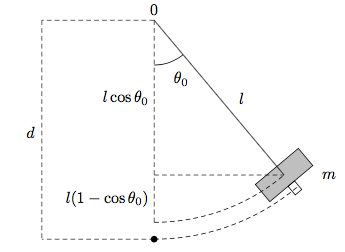
\includegraphics[scale=0.5]{schema_pendolo}
	\newpage
	\section{Analisi Dati}
	\section{Conclusione}
\end{document}